%!TEX root=paper.tex

  \begin{figure*}[h!]
  \centering
  \subfloat[The reported response time (in ms) per deployed version in the observation period]{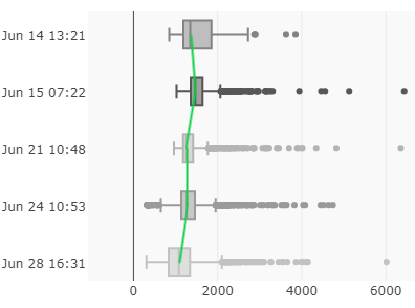
\includegraphics[width=.6\columnwidth]{response_per_version_trunced_trend}}
  \quad
  \subfloat[The measured response time (in ms) using integration with Travis]{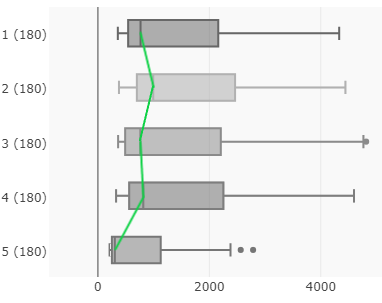
\includegraphics[width=.56\columnwidth]{travis_builds_no_outliers_trend}}
  \caption{Comparison of the response times per endpoint: actual production system versus preemptive monitoring data}
  \label{fig:preemptive}
\end{figure*}


  \section{Preemptive monitoring}

  \ins{INTRO - LINKING WITH PREVIOUS PARAGRAPH: the previous evolutionary view crucial for 
  understanding the impact of software evolution on performance.
  However, just by observing this one can't be sure whether 
  performance changes because of the code or because of the payload.}
  
  \todo{the following might need a bit of rewrite}
  
  The concept of {\em preemptive monitoring} of the application performance by means of instrumenting integration unit testing as the synthetic load is similar to the idea of augmenting service monitoring with online testing~\cite{metzger2010proactive}, i.e.~testing service-based applications by using dedicated test input in parallel to its normal use and operation. The difference is that we take advantage of the capability of the CI framework (i.e. Travis in this case) to create an emulated ``live'' environment for integration testing purposes, and use unit testing as the dedicated test input in order to measure performance. 
  

      \begin{figure}[h!]
        \centering
        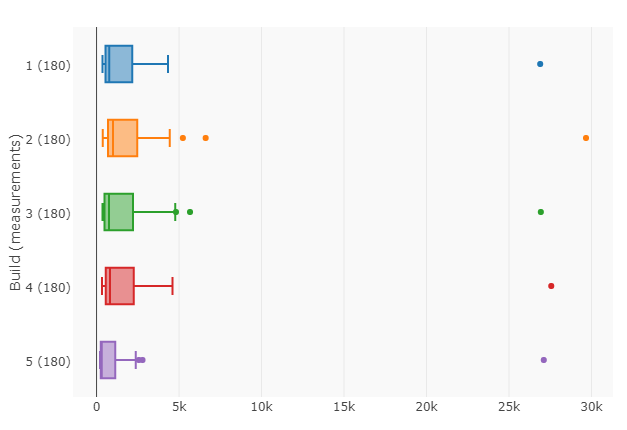
\includegraphics[width=0.7\columnwidth]{travis_builds}
        \caption{Response times in 5 consequent Travis builds in the \zee case study}
        \label{fig:builds}
      \end{figure}



  For example, \Fref{fig:builds} is a screenshot from the dashboard showing the measured response times for 5 consequent builds, with 180 iterations of the unit tests executed in total across all endpoints. The outliers on the right of the figure are due to initial requests \ins{which must wait for a boot-up phase of the API}.  



  
  While this integration testing environment is different from the actual production deployment one, and the load used is purely synthetic, as will show in Section~\ref{sec:evaluation}, it can actually be used successfully as an early performance indicator for the application developer. \ins{Although predicting the performance of the application would require advanced statistical work, it can be succesfully used as an advanced warning system for the overall performance trend for given endpoints}.  


  \paragraph{Integration with Travis}
  \ml{added new section... also, this has to be moved after introducing the pre-emptive monitoring since it's about running tests. switched the order}
  

  \ins{The pre-emptive monitoring system} can be configured to work together with Continuous Integration (CI) frameworks like Travis\footnote{\url{https://travis-ci.org/}} that deal with automated integration testing.
  The developer needs to define the unit test folder of the project, the URL that Travis should use for reporting its results, and the number of iterations for each unit test should be executed in order to generate a load for the application. 
  
  Each time a new build is created through Travis, the \tool automatically detects all available unit tests defined by the application developer and iterates through each one of them the number of times predefined by the developer while monitoring the response times for each request. The resulting measurements are persisted in a separate part of the tool database so as not to contaminate the ``live'' monitoring data. Beyond seeing the results of each Travis build in the \tool, this feature also allows for preemptive monitoring of the application, as we discuss in the following.    

  \ins{Besides functioning as an early warning system for performance, tracking the evolving performance of API tests serves a second purpose. To function as an anchor when the developer analyzes performance degradations. For example, when a developer sees that a given endpoint has become less performant after in a newly deployed version, they are able to investigate whether the performance degradation is visible also with the synthetic load. This would correspond to a performance degradation which is due to ``algorithmic performance degradation''. If on the other hand, the performance of the tests does not change between versions, the developer might conclude that the performance degradation could be due to the workload on the machines, or maybe to the workload mix of the users}
  
  %By these means, an application developer can use unit tests as synthetic loads for driving the performance monitoring of the application before it reaches the production phase.  As we will discuss further in Section~\ref{sec:testing}, this feature is integral in enabling preemptive performance monitoring of the application.  
  

\todo{here goes the discussion about our forecasting capabilities}



\begin{table}[h]
  \begin{tabular}{lll}
    \toprule
    Iteration & \bfseries Live (median) & \bfseries Travis (median)\\
    \midrule
    1 & 1349.41 & 764.87\\ 
    2 & 1466.13 & 992.87\\
    3 & 1256.65 & 760.87\\
    4 & 1266.42 & 813.89\\
    5 & 1080.68 & 303.4\\
    \bottomrule
  \end{tabular}
\end{table}

Pearson correlation $r(3)=.93, p=.02$




    \begin{figure*}[ht!]
      \centering
      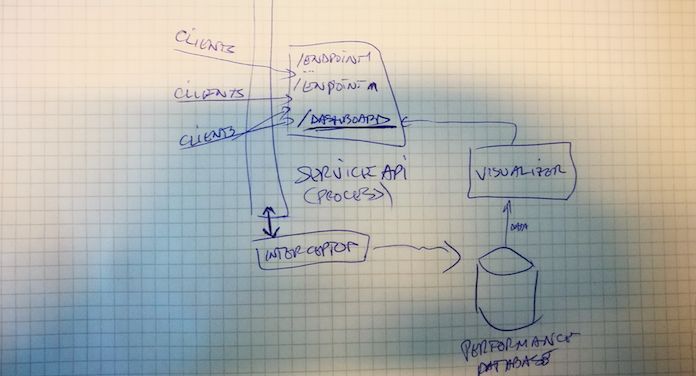
\includegraphics[width=0.8\linewidth]{interceptor}
      \caption{The first thing that needs to be done, is to decorate the application object with an INTERCEPTOR}
      \label{fig:sep}
    \end{figure*}

\newpage
